\chapter{Immagini}

\section{Le immagini digitali}

 Una immagine digitale è definita da un insieme di pixel, ogni pixel rappresenta una informazione che viene campionata e quantizzata (ad esempio il colore è quantizzato, in quanto assume un numero finito di valori) misurata da un sensore. Nota : quantizzare significa quantificare. Lavoreremo molto con le immagini grayscale.
 
 \subsection{Caratteristiche di una immagine}
 \begin{itemize}
 	\item Dimensione (numero di pixel in larghezza  = WxH) e risoluzione(DPI);
 	\item formato dei pixel (possono essere o bianchi o neri oppure a colori)
 	\item formati di memorizzazione e compressione;
 	\item occupazione di memoria di una immagine (si misura in funzione dell'ampiezza per altezza per profondità, in sigla si indica come : WxHxDepth)
 \end{itemize}
 
 \subsection{Immagine greyscale con punti di luce}
 
 Vediamo una immagine come una matrice di punti di luce (ogni elemento della matrice rispetta una scala di luminosità).  Ogni pixel della matrice assume un valore, il quale indica la quantità di luce. 
 \begin{itemize}
 	\item valori più alti : maggiore luminosità
 	\item valori più bassi : minore luminosità
 	\item intervalli tipici : Byte[0, 255] e Float[0 = nero, 1 = luce]
 \end{itemize}

 \subsection{Coordinate dei pixel}
 Ci sono due tipi di coordinate:
 \begin{itemize}
 	\item espresse in forma cartesiana (cv.line(img, (4, 0), (3, 6), color));
 	\item espresse in notazione matriciale (img[3, 1] = x).
 \end{itemize}

\subsection{Organizzazione dei pixel in memoria}

I pixel sono quasi sempre organizzati in memoria per righe, ricordando che la memoria dell'elaboratore non è una matrice, bensì un unico vettore unidimensionale di byte.

\section{OpenCV}

Le immagini le definisco come array numpy bidimensionali. Attenzione imread non ritorna un errore o una eccezione nel caso in cui l'immagine non esista, ritorna un None, occorre dunque fare un controllo.

\begin{lstlisting}
	# creazione di un'immagine grayscale 16x15 con un byte per pixel
	
	img1 = np.zeros((15, 16), dtype=np.uint8) # Tutti i pixel a 0
	img2 = np.full((15, 16), 255, dtype=np.uint8) # Tutti i pixel a 255
	img3 = np.random.randint(0, 256, (15, 16), dtype=np.uint8) # Valori dei pixel casuali
	
	# Caricamento di un'immagine grayscale da file (se e' a colori viene convertita)
	# N.B. se il file non esiste non genera un errore ma restituisce None
	
	#il flag indicato ci dice che anche se l'immagine fosse a colori verrebbe convertita in greyscale
	img4 = cv.imread('esempi/mario.png', cv.IMREAD_GRAYSCALE)
\end{lstlisting}

\begin{figure}[htp]
	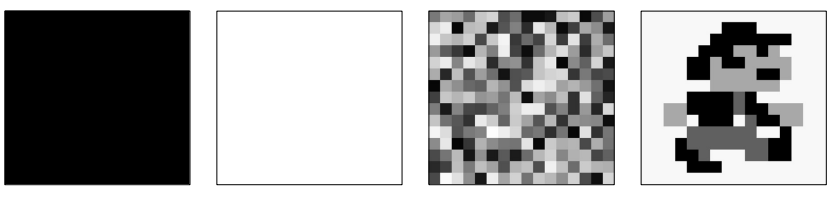
\includegraphics[width=500pt]{./immagini/opencv_images.png}
	\caption{Immagini generate con opencv}
	\label{img:opencv_images}
\end{figure}

\newpage

In seguito viene mostrato come utilizzare slicing e broadcasting per modificare una immagine in python.

\begin{lstlisting}
	a = np.full((15, 16), 255, dtype=np.uint8)	#immagine tutta bianca
	# Slicing e broadcasting
	#partendo dalla terza riga fino alla penultima esclusa, viene fatta la stessa cosa per le colonne
	a[2:-2, 2:-2] = 0		# creo una parte nera, a partire dalla riga di indice 2
	a[4:-4, 4:-4] = 128		# creo una parte grigio chiaro
	a[6:-6, 6:-6] = 64		# grigio con altra tonalita'

	b = a.copy()			
	# Boolean indexing e broadcasting
	mask = b==64 # creo una maschera di bool che conterra' true per tutti i valori di b uguali a 64, dunque sostituisco la parte centrale con il bianco
	b[mask] = 240	#questo array viene esteso attraverso il broadcasting

	c = np.zeros_like(a)	#zeros_like() prende un array e restituisce un array con lo stesso tipo e con le stesse caratteristiche ma tutto a zero
	# Slicing e broadcasting
	c[::2, ::3] = 255

	d = np.zeros((15, 16), dtype=np.uint8)	#immagine nera
	# Integer array indexing e broadcasting
	y = np.array([0, 2, 5, 9, 14])	#array di indici monodimensionale, seleziona le righe sulla quale voglio lavorare
	x = np.arange(0, 16, 2)			#seleziona le colonne che voglio modificare
	#qui sto utilizzando questi array come indici
	d[y[:, np.newaxis], x] = np.arange(50, 255, 50)[:,np.newaxis]
\end{lstlisting}

\begin{figure}[htp]
	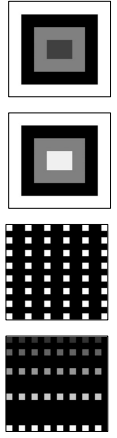
\includegraphics[width=70pt]{./immagini/opencv_images2.png}
	\caption{Immagini generate con opencv}
	\label{img:opencv_images2}
\end{figure}

\section{Immagini a colori: tensori 3D}

Le immagini a colori si modellano mettendo insieme componenti di base (rgb). Una immagine a colori è come se fosse la sovrapposizione di 3 immagini con una determinata scala di valori. Quindi abbiamo che le immagini a colori sono definite da array tridimensionali, la profondità è data dai canali. Sovrapponendosi fra loro dunque, i canali conferiscono il colore all'immagine.

\subsection{Modello RGB}

Ci sono tanti modelli, in questo corso vediamo il minimo indispensabile per capire di cosa si tratti. Il modello di base è l'RGB, è utilizzato ad esempio per generare colore nei monitor, è un modello additivo dal momento che combinando il verde il blu e il rosso si ottiene tutta la varietà di colori. Alla fine abbiamo questi 3 colori ed ogni colore lo possiamo immaginare come un punto in uno spazio tridimensionale (asse del rosso, asse del verde e asse del blu). Per effettuare operazioni di riconoscimento degli oggetti (somiglianza fra colori), lo spazio euclideo del cubo RGB non va bene, perchè i colori che sono simili non sempre sono vicini.

\subsection{Coordinate dei pixel}
Notazione:
\begin{itemize}
	\item cartesiane : pixelpos = (14, 3, 1), sto indicando x, y e canale;
	\item matriciale : img[14, 4, 0], sto indicando r, c, canale.
\end{itemize}

\subsection{Ordine dei canali}

L'ordine dei canali sfruttato normalmente è RGB ma attenzione! Open CV utilizza il modello BGR (B = 0, G = 1, R = 2). In caso di cambio ordine occorre effettuare delle modifiche.

\subsection{Quale è l'ordine dei pixel in memoria?}

Quasi sempre viene utilizzato un canale in modo contiguo. 

\newpage

\section{Caricamento di immagini a colori}

\begin{lstlisting}
	# Creazione di un'immagine 16x20 a 3 canali con valori di tipo byte (3 byte per pixel)

	img1 = np.zeros((20, 16, 3), dtype=np.uint8) # Pixel a 0
	img2 = np.full((20, 16, 3), 255, dtype=np.uint8) # Pixel a 255
	img3 = np.random.randint(0, 256, (20, 16, 3), dtype=np.uint8) # Pixel casuali

	# Caricamento di un'immagine da file (formato BGR)
	# N.B.: se il file non esiste non genera un errore ma restituisce None
	img4 = cv.imread('esempi/mario-c.png')
\end{lstlisting}


\begin{lstlisting}
	# Caricamento di un'immagine da file (formato BGR)
	m = cv.imread('esempi/mario-c.png')
	
	# Crea tre immagini BGR ciascuna con valori solo in un canale e gli altri due a zero
	b, g, r = m.copy(), m.copy(), m.copy()
	#Qui voglio azzerare tutti i canali tranne 1, in modo da ottenere delle immagini monocolore. Lo faccio sfruttando l'ellipsis notation e lo slicing.
	b[...,1:3], g[...,0:3:2], r[...,0:2] = 0, 0, 0
	
	# Crea tre immagini BGR ciascuna corrispondente alla somma di due canali
	c, m, y = b+g, b+r, g+r
\end{lstlisting}

\begin{figure}[htp]
	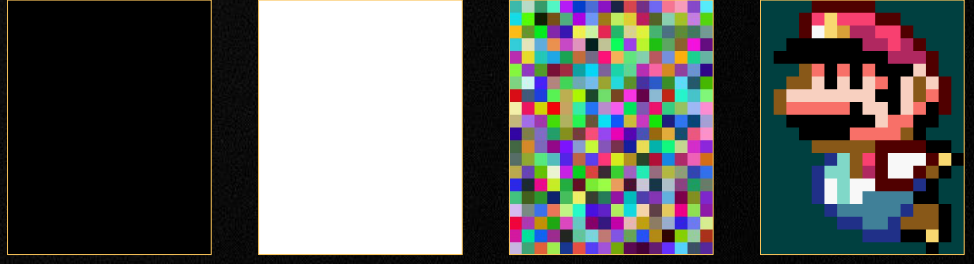
\includegraphics[width=200pt]{./immagini/opencv_images_c1.png}
	\caption{Prime immagini a colori}
	\label{img:opencv_images_c1}
\end{figure}

\begin{figure}[htp]
	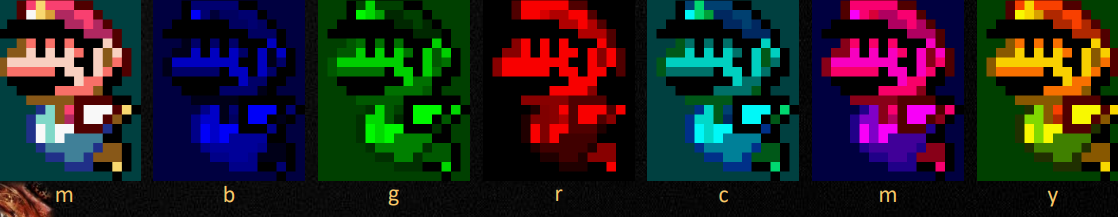
\includegraphics[width=200pt]{./immagini/opencv_images_c2.png}
	\caption{Altre immagini a colori}
	\label{img:opencv_images_c2}
\end{figure}

\newpage

\section{Array numpy tridimensionali}

\begin{figure}[htp]
	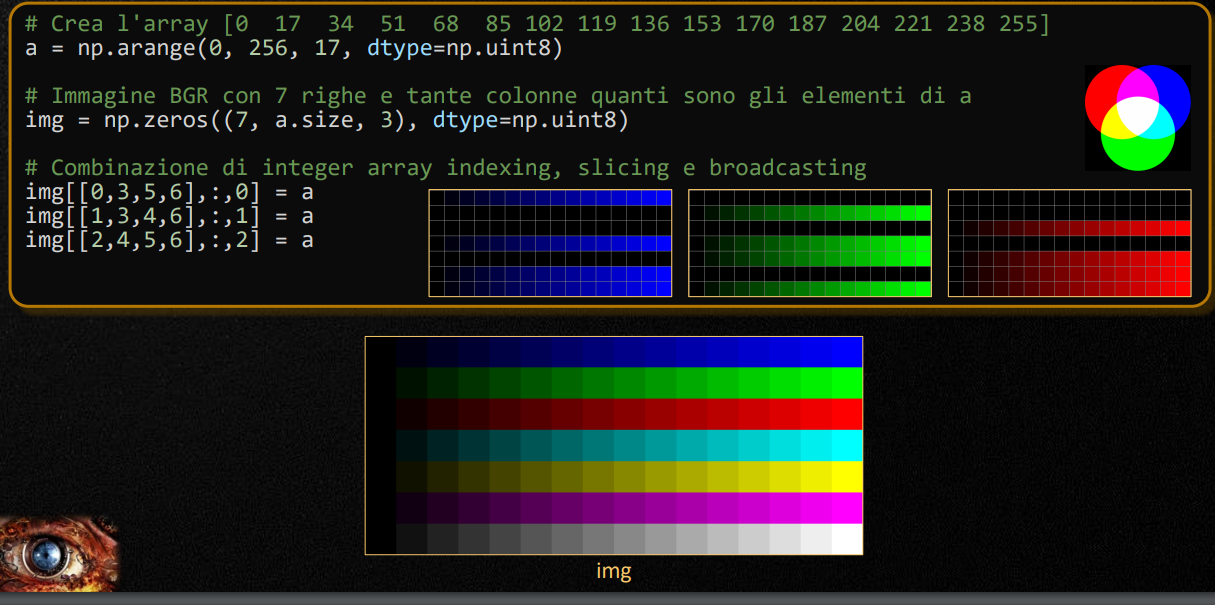
\includegraphics[width=\linewidth]{./immagini/opencv_images_c3.png}
	\label{img:opencv_images_c3}
	\caption{Indicizzazione di array di interi, nell'ultima parte sto dicendo : nel canale 0, su tutte le colonne e su una serie di righe, copio la configurazione definita nel canale a. Faccio la stessa cosa sul canale 1 e 2.}
\end{figure}

\begin{figure}[htp]
	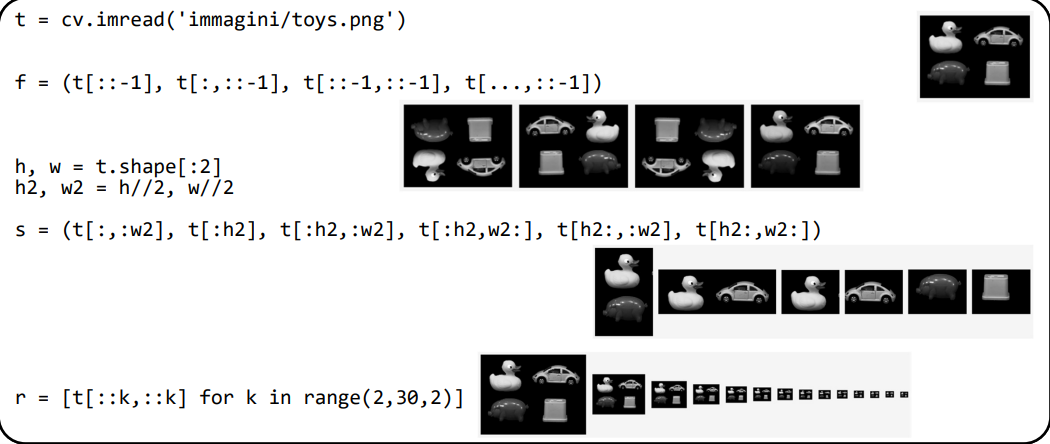
\includegraphics[width=\linewidth]{./immagini/opencv_images_c4.png}
	\caption{Qui utilizziamo lo slicing per fare a fette le immagini. Nel primo caso sto generando una tupla di array numpy}
	\label{img:opencv_images_c4}
\end{figure}

\newpage

\section{Istruzione shape}

\begin{lstlisting}
	t = cv.imread('path')
	
	t.shape #mi mostra la shape dell'immagine : (righe, colonne, canali)
	
	#un amateur fa cosi'...
	
	w = t.shape[1] #numero delle righe
	h = t.shape[0] #numero di colonne
	
	print("Dimensione immagine", w, x, h)
	
	#un super python expert giga chad fa invece cosi'!
	
	h, w, c = t.shape #questo perche' conosco lo scompattamento delle tuple
	
	h, w = t.shape #faccio cosi' se il valore del canale non mi interessa
	
\end{lstlisting}

\section{Rappresentazioni HSV HSL}

Introduciamo due modelli di colori più comodi per noi esseri umani. Sono basate su:
\begin{itemize}
	\item Hue(tinta) : è un angolo;
	\item Saturation(saturazione) :  quanto il colore è bello vivo, va dai colori spenti ai più accesi;
	\item Value o lightness: dice quanta luce c'è nel colore, va dal nero al bianco.
\end{itemize}

\subsection{Differenze HSV e HSL}

In HSV i colori più saturi hanno luminosità 1, mentre nell'HSL 0.5. Ci sono altre caratteristiche che non verranno affrontate nello specifico in questo corso.

\subsection{Modifica ai canali HSL}

Creo un mapping, sfruttando la scala greyscale, fra tutti i possibili angoli (che corrispondono ai colori), consideriamo i valori fra 0 a 255. Per quanto riguarda la saturazione, nel mapping greyscale, si vede in base all'oggetto più luminoso (colore più spento = colore poco saturo, colore più accesi = colore molto saturo). Alla fine della fiera, in questa immagine viene mostrato come determinare i valori H, S ed L attraverso un intelligente mapping  della scala greyscale. Ad esempio, se eseguo una somma sullo HUE sto in realtà ruotando la ruota dei colori, per quello utilizziamo le notazioni in radianti.

\begin{figure}[htp]
	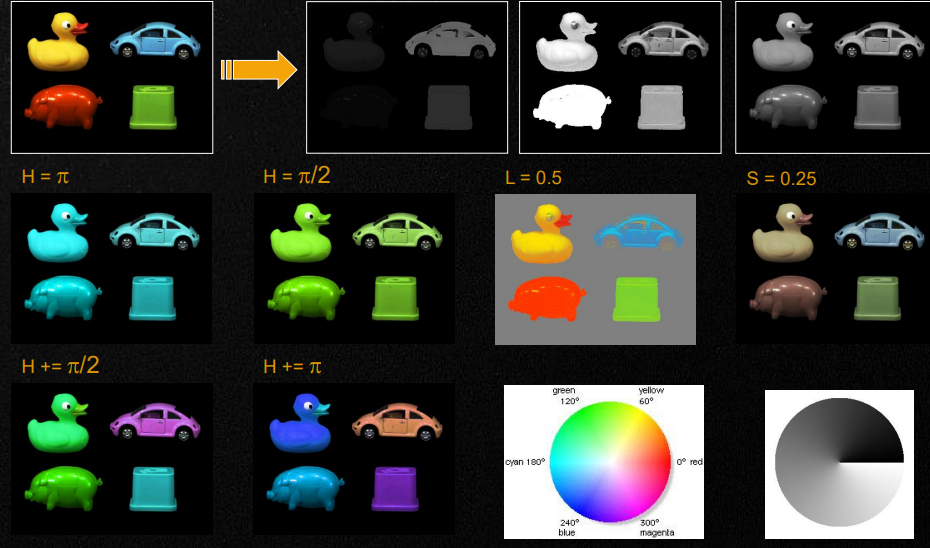
\includegraphics[width=\linewidth]{./immagini/opencv_images_c5.png}
	\caption{Qui utilizziamo lo slicing per fare a fette le immagini. Nel primo caso sto generando una tupla di array numpy}
	\label{img:opencv_images_c5}
\end{figure}

\subsection{HSV e HSL in python/openCV}

La funzione cv.cvtColor(originale, CONV) effettua la conversione del formato del colore, lo si fa specificando una costante come secondo argomento. Attenzione! In python invece di HLS viene considerato HSL.

\begin{lstlisting}
	originale = cv.imread('immagini/toys.png')
	# Converte in HLS
	hls = cv.cvtColor(originale, cv.COLOR_BGR2HLS)
	# Separa i tre canali in 3 immagini grayscale
	h, l, s = cv.split(hls)
	
	# Modifica alcuni dei valori HLS
	# Dimezza la luminosita' di tutti i pixel
	
	l1 = l//2
	
	# Valore di saturazione 64 per tutti i pixel
	
	s1 = np.full_like(s, 64)
	
	# Riunisce i canali e converte in BGR
	#merge e' il corrispettivo di merge, vuole un solo parametro e deve essere una tupla
	
	risultato = cv.cvtColor(cv.merge((h, l1, s1) 
\end{lstlisting}

\begin{figure}[htp]
	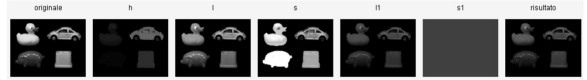
\includegraphics[width=300pt]{./immagini/opencv_images_c6.png}
	\label{img:opencv_images_c6}
\end{figure}

\begin{lstlisting}
	s = [0, 64, 128, 192, 255] # 5 livelli di saturazione
	
	# 18 valori di luminosita' in ogni colonna, np.tile permette di replicare tutte le volte che voglio un array, creando un array piu' grande
	v = np.tile(np.arange(255, -1, -15, np.uint8)[:,np.newaxis], (1, 18))
	
	# 18 valori di hue in ogni riga
	h = np.tile(np.arange(0, 180, 10, np.uint8), (18, 1))
	
	# Combina i 3 canali (si poteva usare anche cv.merge)
	hsv = [np.dstack((h, np.full_like(h, x), v)) for x in s]
	hls = [i[...,[0,2,1]] for i in hsv] # Scambia gli ultimi due canali
\end{lstlisting}


\begin{figure}[htp]
	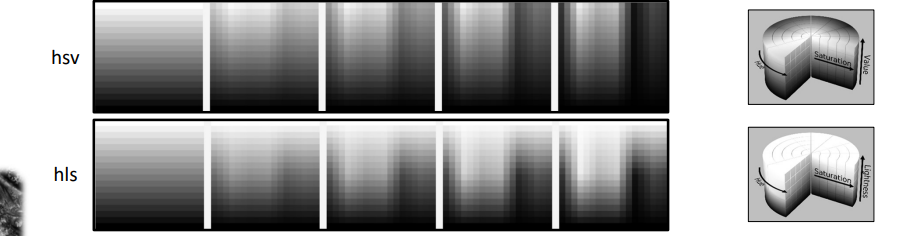
\includegraphics[width=\linewidth]{./immagini/opencv_images_c7.png}
	\label{img:opencv_images_c7}
\end{figure}
